\documentclass[letterpaper,12pt,titlepage,oneside,final]{book}
\newcommand{\package}[1]{\textbf{#1}} 
\newcommand{\cmmd}[1]{\textbackslash\texttt{#1}} 
\newcommand{\href}[1]{#1}

\usepackage{listings}
\lstset{language=Matlab}
\lstset{breaklines}
\lstset{extendedchars=false}

\usepackage{ifthen}
\newboolean{PrintVersion}
\setboolean{PrintVersion}{false} 
\usepackage{amsmath,amssymb,amstext}
\usepackage{algorithm}
\usepackage{algorithmic}
\usepackage[pdftex]{graphicx} 
\usepackage[pdftex,letterpaper=true,pagebackref=false]{hyperref}
\hypersetup{
    plainpages=false,       % needed if Roman numbers in frontpages
    pdfpagelabels=true,     % adds page number as label in Acrobat's page count
    bookmarks=true,         % show bookmarks bar?
    unicode=false,          % non-Latin characters in Acrobat’s bookmarks
    pdftoolbar=true,        % show Acrobat’s toolbar?
    pdfmenubar=true,        % show Acrobat’s menu?
    pdffitwindow=false,     % window fit to page when opened
    pdfstartview={FitH},    % fits the width of the page to the window
    pdftitle={Report for Simulated Annealing and Trust-Region Method with Smoothing Techniques},    % title: CHANGE THIS TEXT!
    pdfauthor={Yichen Zhang},    % author: CHANGE THIS TEXT! and uncomment this line
    pdfsubject={Report for Simulated Annealing and Trust-Region Method with Smoothing Techniques},  % subject: CHANGE THIS TEXT! and uncomment this line
%    pdfkeywords={keyword1} {key2} {key3}, % list of keywords, and uncomment this line if desired
    pdfnewwindow=true,      % links in new window
    colorlinks=true,        % false: boxed links; true: colored links
    linkcolor=blue,         % color of internal links
    citecolor=green,        % color of links to bibliography
    filecolor=magenta,      % color of file links
    urlcolor=cyan           % color of external links
}
\ifthenelse{\boolean{PrintVersion}}{   % for improved print quality, change some hyperref options
\hypersetup{	% override some previously defined hyperref options
%    colorlinks,%
    citecolor=black,%
    filecolor=black,%
    linkcolor=black,%
    urlcolor=black}
}{} 
\setlength{\marginparwidth}{0pt} 
\setlength{\marginparsep}{0pt} 
\setlength{\evensidemargin}{0.125in} 
\setlength{\oddsidemargin}{0.125in} 
\setlength{\textwidth}{6.375in} 

\raggedbottom
\setlength{\parskip}{\medskipamount}
\renewcommand{\baselinestretch}{1} 
\let\origdoublepage\cleardoublepage
\newcommand{\clearemptydoublepage}{
\clearpage{\pagestyle{empty}\origdoublepage}}
\let\cleardoublepage\clearemptydoublepage

\begin{document}

\chapter{Smoothing Techniques}

\section{Reasons for Smoothing}

Sometimes the function is very nasty and has many local optima, so it is very difficult for Trust-Region or Simulated Annealing to find the global one. The smoothing technique can help simulated annealing to find the global optimum more efficiently. By efficiently, we mean take a little longer time and get a much better answer.

\begin{figure}[H]
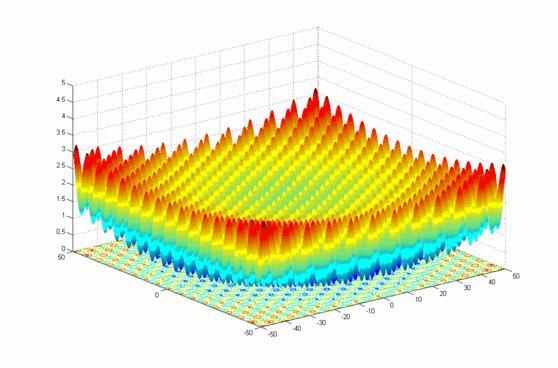
\includegraphics[scale=0.55]{griewank.jpg}
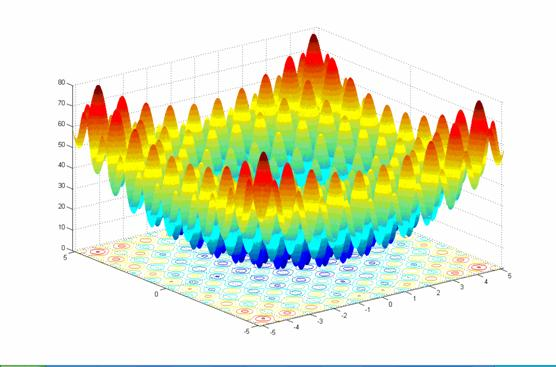
\includegraphics[scale=0.55]{Rastrigin.jpg}
\caption{Griewank and Rastrigin function}
\end{figure}

\section{Two Ways for Smoothing}

\begin{itemize}

\item $\bar{f}(x)=f(x)+\frac{1}{6}\Delta^2trace(H)$

\item $\bar{f}(x)=f(x)+\lambda||x-x_*||_2^2$

\end{itemize}

Where $H$ is the Hessian matrix and $x_*$ is the global optimum we guess. $\Delta$ and $\lambda$ is defined by user.

We call the first one \emph{Trace-Smooth} and the second one \emph{$\lambda$-Smooth}

Now we state the derivation of the formula: $\bar{f}(x)=f(x)+\frac{1}{6}\Delta^2trace(H)$.

Let $f$ be an objective function and $\Delta$ be a positive number. The average value of $f$ over a regular
$\Delta$-box $Box(x)$ centred at $x$ with sides $[x_i-\Delta ,x_i+\Delta ]$ is:

\begin{equation} \label{eq1}
\bar{f}(x)=\frac{1}{(2\ast\Delta)^n}\int_{Box(x)}f(x)dx_1...dx_n
\end{equation}

The formula above is too expensive to compute when $n$ is large or function $f$ is difficult to
compute. However, by approximating $f$ using quadratic Taylor series expansion

\begin{equation}
f(x+s)\cong f(x)+g^Ts+\frac{1}{2}s^THs\equiv q(x)
\end{equation}

where $g=\triangledown f(x)$, $H=\triangledown^2f(x)$ ,\ref{eq1} can be approximated as

\begin{equation}
\bar{f}(x)\cong \bar{q}(x)=f(x)+\frac{1}{(2\ast\Delta)^n}\int_{\forall i,|s_i|\leq\Delta}(g^Ts+\frac{1}{2}s^THs)ds_1...ds_n
\end{equation}

Since 

\begin{equation}
g^Ts+\frac{1}{2}s^THs=\sum_ig_is_i+\sum_i\sum_js_is_jh_{ij}
\end{equation}

Interchanging the order of summation and integration of the above formula yields:

\begin{equation}
\bar{f}(x)=f(x)+\frac{1}{6}\Delta^2\cdot trace(H)
\end{equation}

\section{The Pictures of $Trace-Smooth$ Technique}

Here we give 4 examples for using the smoothing technique $\bar{f}(x)=f(x)+\frac{1}{6}\Delta^2\cdot trace(H)$.

\begin{figure}[H]
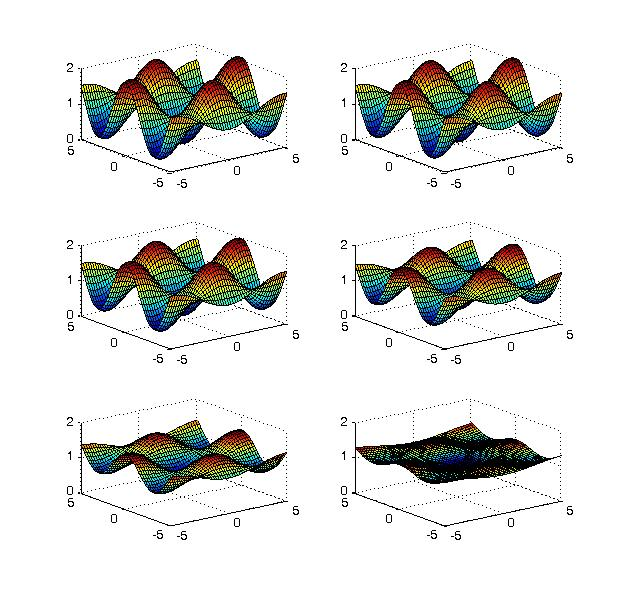
\includegraphics[scale=0.75]{smoothgriewank.jpg}
\caption{Griewank Smoothing}
\end{figure}

\begin{figure}[H]
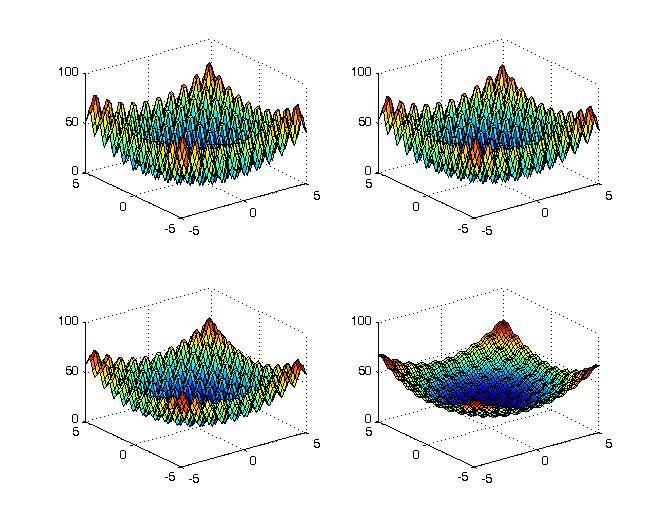
\includegraphics[scale=0.75]{smoothrast.jpg}
\caption{Rastrigin Smoothing}
\end{figure}

\begin{figure}[H]
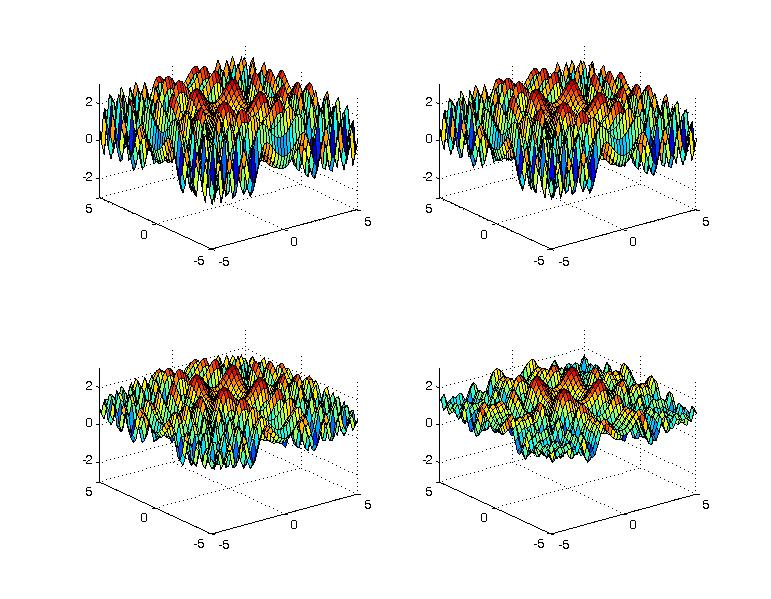
\includegraphics[scale=0.65]{smooth2.jpg}
\caption{Smoothing for $f(x,y)=1+\sin x^2+\sin y^2-0.1e^{-x^2-y^2}$ (Example from CGO)}
\end{figure}

\begin{figure}[H] 
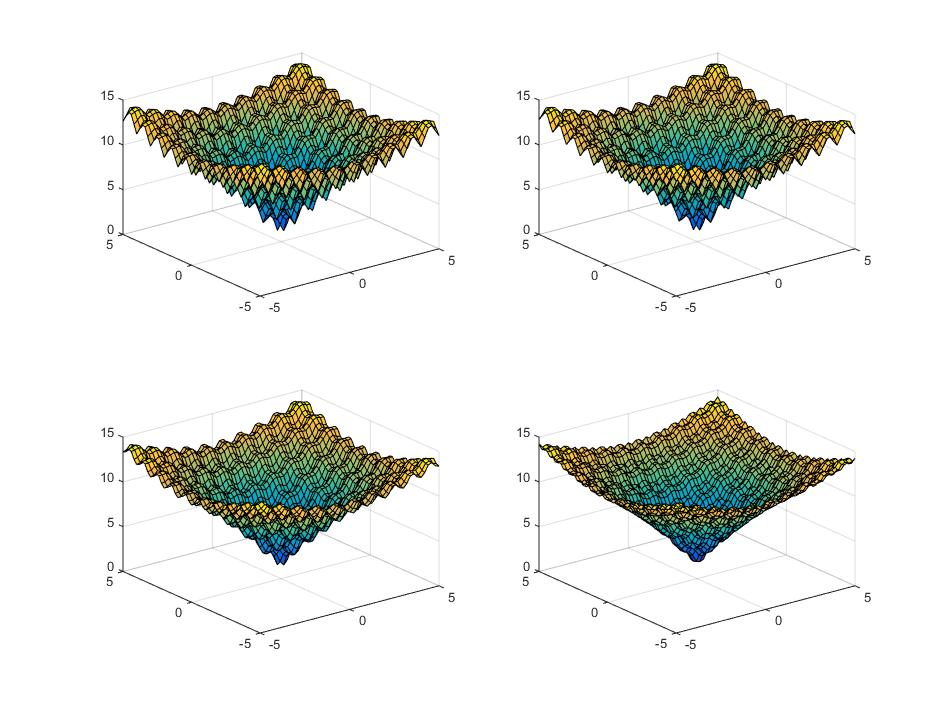
\includegraphics[scale=0.5]{smoothackley.jpg}
\caption{Ackley Smoothing}\label{sac} 
\end{figure}

\section{Original Smoothing Algorithm and Our Modified Smoothing Techniques}

In CGO, Simulated Annealing with Smoothing Algorithm is:

\begin{algorithm} [H]
\caption{Simulated Annealing with Smoothing in CGO}
\begin{algorithmic} 
\STATE Given $Ts, L, Kb, \Delta$ sequence:$Ds$, $x_0$
\FOR { $ k =1,...length(Ts)$ }
\STATE $L$ = number of moves to attempt, $T= Ts(k)$, $\Delta=Ds(k)$.
\STATE Search region $sr=(-lb+ub)*\frac{T}{\max(Ts)}$
\FOR { $ m =1\ \mbox{to} \ L$ }
\STATE Randomly generate a new neighbouring solution $x_{new}$ in $[x_{old}-sr,x_{old}+sr]$ and make sure that $x_{new}$ does not exceed the boundaries.
\STATE Evaluate $\bar{f}_{new}=f(x_{new})+\frac{1}{6}\Delta^2trace(H)$.
\IF{ $\bar{f}_{new} < \bar{f}_{old}$} 
\STATE Accept this new solution, and update the solution. 
\ELSE 
\STATE Accept with probability $P(T) = e^{\frac{-(\bar{f}_{new}-\bar{f}_{old})}{Kb\cdot T} }$. 
\STATE  Update the solution if accepted.
\ENDIF
\ENDFOR
\ENDFOR
\end{algorithmic}
\end{algorithm}

We did two modifications for this algorithm:

\begin{itemize}

\item First, instead of letting temperature sequence and $\Delta$ sequence have the same length, we let the $\Delta$ sequence contains only several entries depends on the problem. For each entry in the $\Delta$ sequence, we run through all the temperature sequence and use the result for the next entry of $\Delta$ sequence.

\item Second, we add a $srmin$ parameter to control the search region does not become too small. Cause if we use $Ts=T_0*0.9^{0:199}$ for example, $0.9^{199}=7.8\times 10^{-10}$, $0.9^{99}=2.95\times 10^{-5}$ so basically after running 99 entries in $Ts$, the search region is less than $(-lb+ub)*2.95\times 10^{-5}$ so the point almost stay the same for the last 100 entries of $Ts$.

\end{itemize}

So our new Simulated Annealing with Smoothing Technique Algorithm is:

\begin{algorithm} [H]
\caption{Modified Simulated Annealing with $Trace-Smooth$}
\begin{algorithmic} 
\STATE Given $Ts, L, Kb, \Delta$ sequence:$Ds$, $x_0, srmin$
\FOR { $ i =1,...length(Ds)$ }
\STATE $\Delta=Ds(i)$
\FOR { $ k =1,...length(Ts)$ }
\STATE $L$ = number of moves to attempt, $T= Ts(k)$.
\STATE Search region $sr=\max\{(-lb+ub)*\frac{T}{\max(Ts)},srmin\}$
\FOR { $ m =1\ \mbox{to} \ L$ }
\STATE Randomly generate a new neighbouring solution $x_{new}$ in $[x_{old}-sr,x_{old}+sr]$ and make sure that $x_{new}$ does not exceed the boundaries.
\STATE Evaluate $\bar{f}_{new}=f(x_{new})+\frac{1}{6}\Delta^2trace(H)$.
\IF{ $\bar{f}_{new} < \bar{f}_{old}$} 
\STATE Accept this new solution, and update the solution. 
\ELSE 
\STATE Accept with probability $P(T) = e^{\frac{-(\bar{f}_{new}-\bar{f}_{old})}{Kb\cdot T} }$. 
\STATE  Update the solution if accepted.
\ENDIF
\ENDFOR
\ENDFOR
\ENDFOR
\end{algorithmic}
\end{algorithm}

The numerical results show that our modifications made the simulated annealing more efficient and can do better than before. 

\begin{figure}[H]
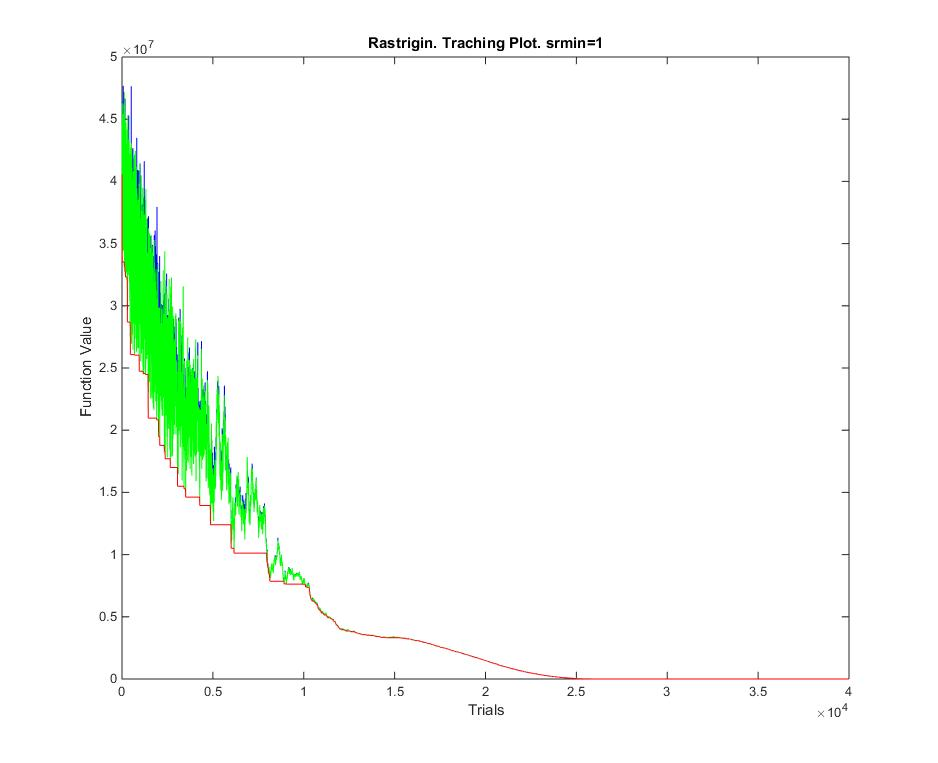
\includegraphics[scale=0.5]{srmin1.jpg}
\caption{Rastrigin. Tracking Plot. srmin=1.}
\end{figure}

\begin{figure}[H]
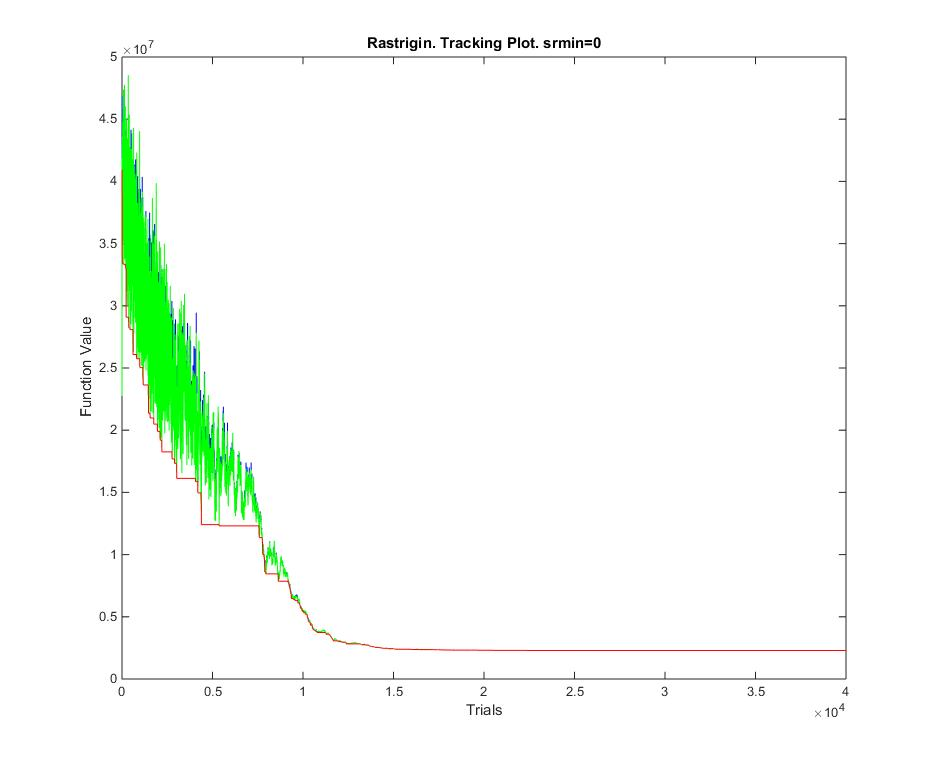
\includegraphics[scale=0.5]{srmin2.jpg}
\caption{Rastrigin. Tracking Plot. srmin=0 (original).}
\end{figure}

srmin should be defined according to the search range of the problem. Also you can set it to 0 to use the original search range in CGO.

Similarly, the algorithm of simulated annealing with $\lambda-Smooth$ is:

\begin{algorithm} [H]
\caption{Modified Simulated Annealing with $\lambda-Smooth$}
\begin{algorithmic} 
\STATE Given $Ts, L, Kb, \lambda$ sequence:$Ls$, $x_0, x_*, srmin$
\FOR { $ i =1,...length(Ds)$ }
\STATE $\lambda=Ls(i)$
\FOR { $ k =1,...length(Ts)$ }
\STATE $L$ = number of moves to attempt, $T= Ts(k)$.
\STATE Search region $sr=\max\{(-lb+ub)*\frac{T}{\max(Ts)},srmin\}$
\FOR { $ m =1\ \mbox{to} \ L$ }
\STATE Randomly generate a new neighbouring solution $x_{new}$ in $[x_{old}-sr,x_{old}+sr]$ and make sure that $x_{new}$ does not exceed the boundaries.
\STATE Evaluate $\bar{f}_{new}=f(x_{new})+\lambda||x-x_*||_2^2$.
\IF{ $\bar{f}_{new} < \bar{f}_{old}$} 
\STATE Accept this new solution, and update the solution. 
\ELSE 
\STATE Accept with probability $P(T) = e^{\frac{-(\bar{f}_{new}-\bar{f}_{old})}{Kb\cdot T} }$. 
\STATE  Update the solution if accepted.
\ENDIF
\ENDFOR
\ENDFOR
\ENDFOR
\end{algorithmic}
\end{algorithm}

Notice that simulated annealing is phase 1. For phase 2 we use $fmincon$ with start point(s) came from phase 1 to get the final results.

\chapter{Numerical Results}

We use three problems which have many local optima and are very difficult to find the global optimum. They are:

\begin{itemize}

\item Griewank

\item Rastrigin

\item Ackley

\end{itemize}

And test the four methods:

\begin{itemize}

\item Simulated Annealing with $Trace-Smooth$

\item Simulated Annealing with $\lambda-Smooth$

\item Pure Simulated Annealing

\item MATLAB build-in function $fmincon$ (Trust-Region)

\end{itemize}

We set up the same parameters for the 3 SA methods and use same start point for 4 methods.

\section{Griewank}

Griewank function is:

\begin{equation}
f(x)=p* \sum_{i=1}^n x_i^2-\prod_{i=1}^n \cos \left(\frac{x_i}{\sqrt{i}}\right)+1
\end{equation}

Usually $p=\frac{1}{4000}$ and we can control $p$ to control the shape of the function.\\
It has many local optima and the global one is $x_*=[0,0,...,0]^T$, $f(x_*)=0$.

\begin{figure}[H]
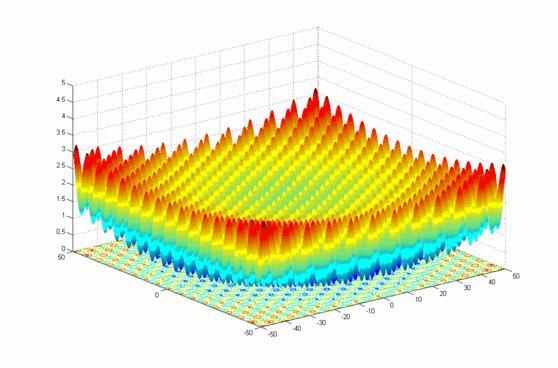
\includegraphics[scale=1.1]{griewank.jpg}
\caption{Griewank}
\end{figure}

We use a randomly generated $x_*$ from $[-1,-1,...,-1]^T$ to $[1,1,...,1]^T$. Although we know the exact value of $x_*$ but we pretend we don't know to be fair for other methods. The search region is from $[-1000,-1000,...,-1000]^T$ to $[1000,1000,...,1000]^T$.

We did 20 cases using different start point for $n=6$ and $p=\frac{1}{4000}$ of Griewank. $x-axis$ is the number of cases and $y-axis$ is the final function value. 

\begin{figure}[H]
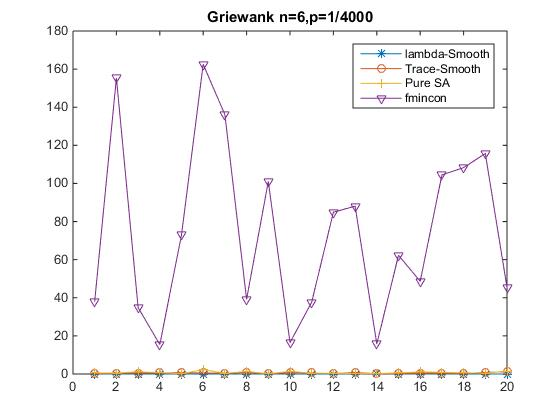
\includegraphics[scale=0.7]{griewank1.jpg}
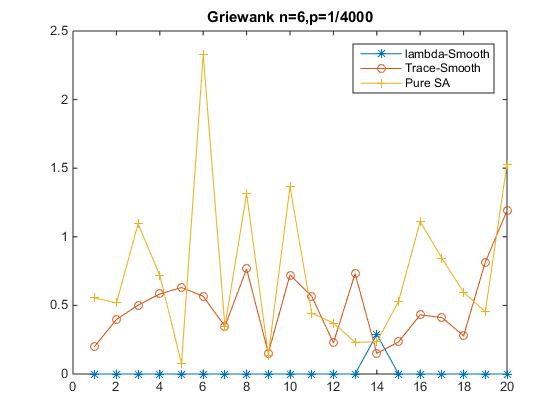
\includegraphics[scale=0.7]{griewank2.jpg}
\caption{Compare SA Methods with $fmincon$}
\end{figure}

The first figure shows that the three simulated annealing methods are better than just use $fmincon$ cause Griewank function is very hard for $fmincon$(Trust-Region) to solve.

The second figure we remove the $fmincon$ line to compare our three simulated annealing methods. We can see that our $\lambda-Smooth$ is doing best and $Trace-Smooth$ is better than pure simulated annealing in most cases(16 out of 20).

As we mentioned before, we can control the value of $p$ to change the shape of Griewank.

\begin{figure}[H]
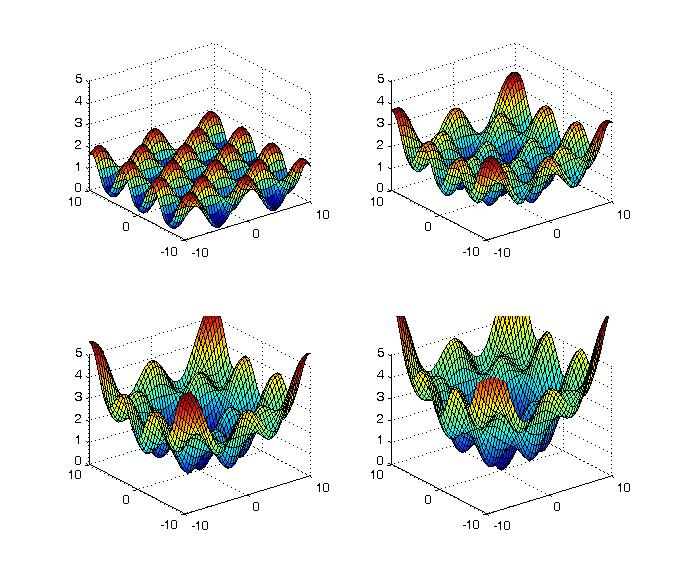
\includegraphics[scale=0.6]{diffp.jpg}
\caption{Shape of Griewank if $p$ becomes greater}
\end{figure}

\begin{figure}[H]
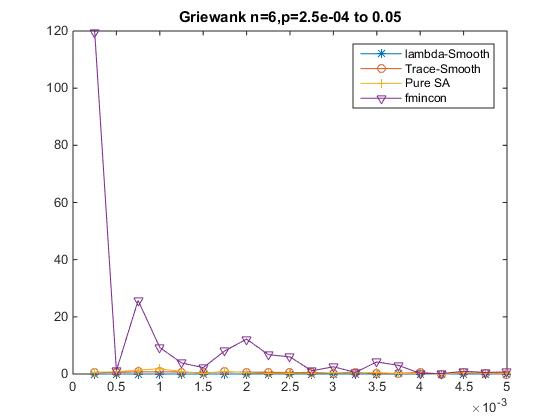
\includegraphics[scale=0.7]{griewank3.jpg}
\caption{Compare SA methods with $fmincon$ when function becomes flattened}
\end{figure}

$x-axis$ is the value of $p$ and $y-axis$ is the final function value.

As $p$ goes greater, the function shape is more flattened. So $fmincon$ can do better because the function is not so nasty. In this situation the results of $fmincon$ and our 3 SA methods doesn't show much difference.

\section{Rastrigin}

Rastrigin function is:

\begin{equation}
f(x)=10n+\sum_{i=1}^n(x_i^2-10\cos (2\pi x_i))
\end{equation}

The global optima is $x_*=[0,0,...,0]^T$ and $f(x_*)=0$.

As $n$ goes bigger, it is very difficult to find the global optima using simulated annealing or trust-region.

\begin{figure}[H]
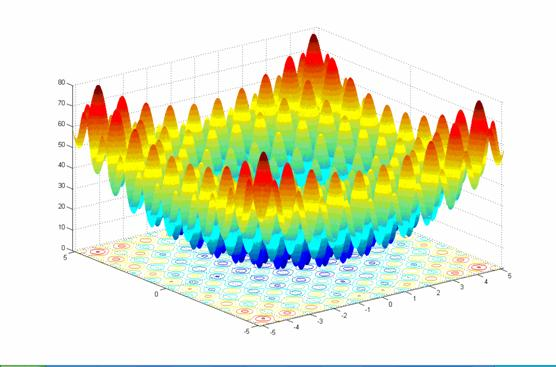
\includegraphics[scale=1.1]{Rastrigin}
\caption{Rastrigin}
\end{figure}

In this example we use $n$ from 55 to 150 to see the difference of each method. Same as we did in Griewank example, we use a randomly generated $x_*$ from $[-1,-1,...,-1]^T$ to $[1,1,...,1]^T$. The search region is from $[-1000,-1000,...,-1000]^T$ to $[1000,1000,...,1000]^T$. 

$x-axis$ is dimension $n$ and $y-axis$ is the final function value.

First two figures are the result for the comparison of four methods.

The last two figures are the results and time we compare our three simulated annealing methods with MATLAB build-in SA function: $simulannealbnd$. 

\begin{figure}[H]
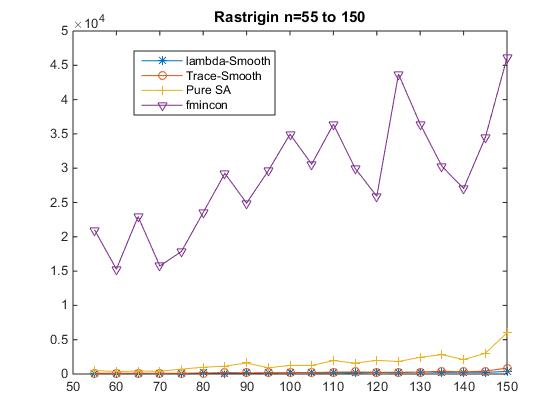
\includegraphics[scale=0.7]{rast1.jpg}
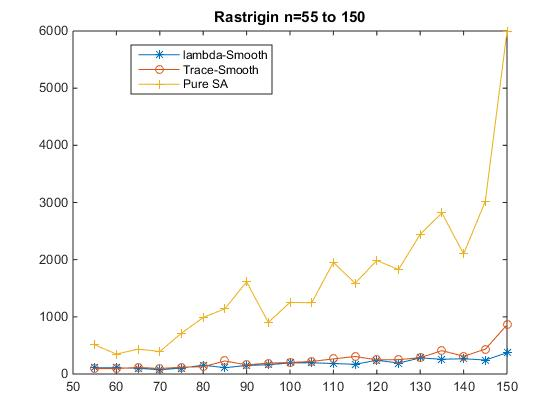
\includegraphics[scale=0.7]{rast2.jpg}
\caption{Compare SA Methods with $fmincon$}
\end{figure}

\begin{figure}[H]
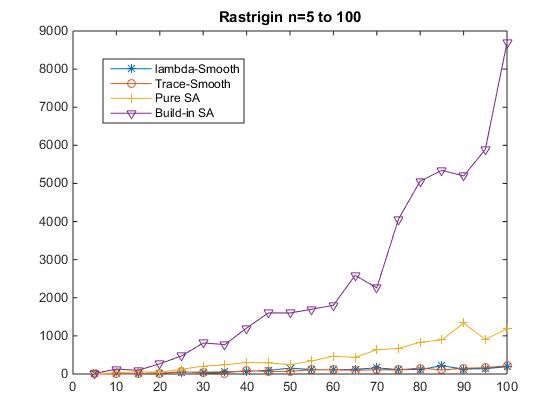
\includegraphics[scale=0.7]{rast4.jpg}
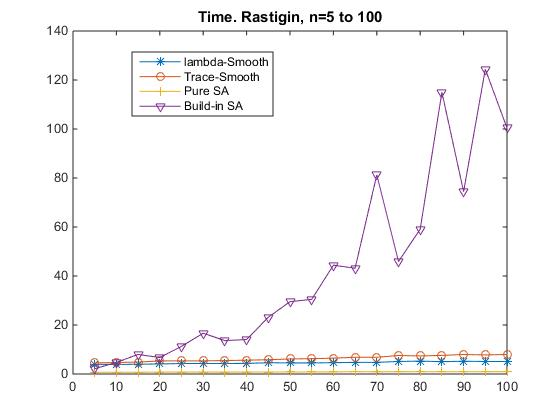
\includegraphics[scale=0.7]{rast5.jpg}
\caption{Compare Our 3 SA Methods with MATLAB Build-in SA function}
\end{figure}

From the first two figures we can see clearly that our smoothing techniques really work cause they can get a much better results than just using the pure simulated annealing.

From the last two figures we can see that our simulated annealing code is much more efficient than MATLAB build-in function. We take less time and get better answer. The reason probably is that $simulannealbnd$ only input the function handle, $x_0$, upper and lower bound but no other parameters.

\section{Ackley}

The Ackley function is:

\begin{equation}
f(x)=20+e-20e^{-\frac{1}{5}\sqrt{\frac{1}{n}\sum_{i=1}^nx_i^2}}-e^{\frac{1}{n}\sum_{i=1}^n\cos(2\pi x_i)}
\end{equation}

\begin{figure}[H]
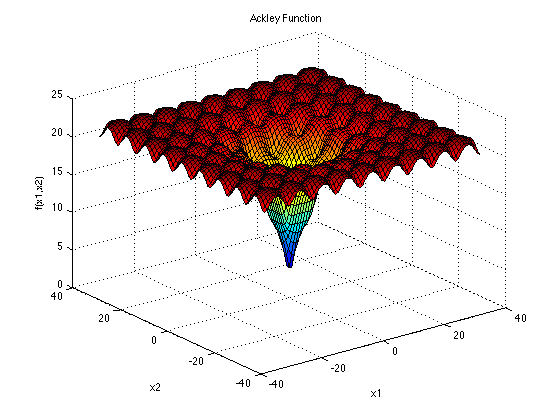
\includegraphics[scale=0.75]{ackley.png}
\caption{Ackley function for $n=2$}
\end{figure}

There are many local optima and one global optimum at $x_*=[0,0,...,0]^T$. $f(x_*)=0$. However, as $n$ goes bigger, it is very difficult to find the global optimum. The search region is: $[-30,-30,...,-30]^T$ to $[30,30,...,30]^T$. 

$x-axis$ is the dimension $n$ and $y-axis$ is the final function value.

\begin{figure}[H]
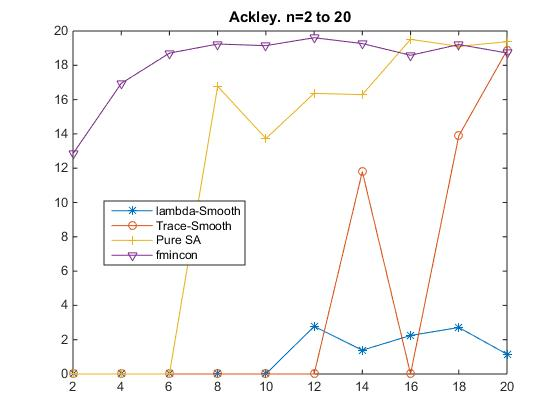
\includegraphics[scale=0.7]{ackley1.jpg}
\caption{Ackley example. $n=2$ to $20$}
\end{figure}

For this example, first we can say that $\lambda-Smooth$ doing well as usual. However, $Trace-Smooth$ is not so stable and we think that is probably because we didn't set the $\Delta$-sequence right. For the previous examples, we did lots of experiments to find the suitable $\Delta$-sequence for each problem. But this time we use $ADMAT$ to compute $H$ and it takes quite a long time to run the $Trace-Smooth$ simulated annealing(Took 3.5 hours to get this figure). We believe that $Trace-Smooth$ technique can do better if we set up the right $\Delta$-sequence since the picture we showed in figure \ref{sac} illustrates that $Trace-Smooth$ technique can smooth the Ackley function very well.

\chapter{Trust-Region Method with Simulated Annealing and Smoothing Technique}

\section{Introduction}

We have tested the Trust-Region Method combined with Simulated Annealing and found it is an improvement over just using Trust-Region Method (see another report for detail). Now we want to combine Trust-Region Method with Simulated Annealing and Smoothing Technique. 

For Trust-Region Method, we need to compute gradient $g$ and Hessian matrix $H$ to solve the Trust-Region sub-problem for each iteration. 

For $\lambda-Smooth$, $\bar{f}(x)=f(x)+\lambda||x-x_*||_2^2$, since $||x-x_*||_2^2=\sum_{i=1}^n(x_i-x_{*i})^2$. So we have:

\begin{equation}
\bar{g}=g+2\lambda(x-x_*)
\end{equation}

\begin{equation}
\bar{H}=H+2\lambda I
\end{equation} 

Where $g$ and $H$ is the gradient and Hessian matrix of original function $f(x)$.

For $Trace-Smooth$ $\bar{f}(x)=f(x)+\frac{1}{6}\Delta^2trace(H)$, since $trace(H)=\sum_{i=1}^n\frac{\partial^2 f}{\partial x_i^2}$. So we have:

\begin{equation}
\bar{g}=g+\frac{1}{6}\Delta^2\sum_{k=1}^n\frac{\partial^3 f}{\partial x_k^2\partial x_i}
\end{equation}

\begin{equation}
\bar{H}=H+\frac{1}{6}\Delta^2R
\end{equation} 

Where $g$ and $H$ is the gradient and Hessian matrix of original function $f(x)$ and matrix $R$ is:

\begin{equation}
R_{ij}=\sum_{k=1}^n\frac{\partial^4 f}{\partial x_k^2\partial x_i\partial x_j}
\end{equation}

Since usually we can not get the information of the third and forth derivation, so we decide just use the original function $f(x)$'s gradient and Hessian matrix for each iteration and use the formula $\bar{f}(x)=f(x)+\frac{1}{6}\Delta^2trace(H)$ to compute the function's value. Now we give the four algorithms for Trust-Region method with simulated annealing and smoothing techniques.

\begin{algorithm} [H]
\caption{Trust Region Method (TRM)}
\begin{algorithmic} 
\STATE Given $\tau_1, \tau_2, \gamma1, \gamma2$
\WHILE {$norm(g)>tol$ and number of iterations$<itbnd$}
\STATE  Solve TRS for $s_k$, assign $qpval_k \leftarrow \triangledown  f^T_ks_k+\frac{1}{2}s^T_k \triangledown^2f_ks_k$
\STATE  $newval_k\leftarrow f(x_k+s_k)$
\STATE  $ratio_k\leftarrow \frac{newval_k-f_k}{qpval_k}$
\STATE  Adjust $\Delta_k$
\IF{ $ratio_k< \tau_1$} 
\STATE $\Delta_{k+1}\leftarrow \frac{||s_k||}{\gamma_1}$
\ELSE 
\IF{$ratio_k>\tau_2$,and $||s_k||=\Delta_k$}
\STATE $\Delta_{k+1}\leftarrow \gamma_2 \Delta_k$
\ELSE 
\STATE $\Delta_{k+1}\leftarrow \Delta_k$
\ENDIF
\ENDIF
\STATE Update $x$:
\IF {$ratio_k\leq 0$}
\STATE $x_{k+1}\leftarrow x_k$
\ELSE 
\STATE $x_{k+1}\leftarrow x_k+s_k$
\ENDIF
\ENDWHILE
\end{algorithmic}
\end{algorithm}


\begin{algorithm} [H]
\caption{Trust-Region Method with Simulated Annealing }
\begin{algorithmic} 
\STATE Given temperature sequence $T$, $Trials$, $x_0$, $m=0$
\STATE \emph{Phase 1:}
\FOR { $ n =1,...,length(T)$ }
\STATE Given $\tau_1, \tau_2, \gamma1, \gamma2$, $t=T(n)$, $x=x_0$
\WHILE {$norm(g)>tol$ and number of iterations$<Trials$}
\STATE  Solve TRS for $s_k$, assign $qpval_k \leftarrow \triangledown  f^T_ks_k+\frac{1}{2}s^T_k \triangledown^2f_ks_k$
\STATE  $newval_k\leftarrow f(x_k+s_k)$
\STATE  $ratio_k\leftarrow \frac{newval_k-f_k}{qpval_k}$
\STATE  Adjust $\Delta_k$
\IF{ $ratio_k< \tau_1$} 
\STATE $\Delta_{k+1}\leftarrow \frac{||s_k||}{\gamma_1}$
\ELSE 
\IF{$ratio_k>\tau_2$,and $||s_k||=\Delta_k$}
\STATE $\Delta_{k+1}\leftarrow \gamma_2 \Delta_k$
\ELSE 
\STATE $\Delta_{k+1}\leftarrow \Delta_k$
\ENDIF
\ENDIF
\STATE Update $x$:
\IF {$ratio_k\geq 0$ or $exp(\frac{ratio_k}{t})>rand$}
\STATE $x_{k+1}\leftarrow x_k+s_k$
\ELSE 
\STATE $x_{k+1}\leftarrow x_k$
\ENDIF
\ENDWHILE
\STATE $f_n=f(x_k)$
\IF{ $f_n$ is different from any $f_1$ to $f_{n-1}$} 
\STATE $m=m+1$, $\overline{x_m}=x_k$, ;
\ENDIF
\ENDFOR
\STATE  
\STATE \emph{Phase 2:}
\FOR {$k=1,...,m$}
\STATE Algorithm 4 with initial point $\overline{x_k}$
\ENDFOR
\STATE Output the smallest $f$ in phase 2 and its point.
\end{algorithmic}
\end{algorithm}

\begin{algorithm} [H]
\caption{Trust-Region Method with Simulated Annealing and $\lambda-Smooth$}
\begin{algorithmic} 
\STATE Given temperature sequence $T$, $Trials$, $x_0$, $m=0$, $x_*$, $\lambda$ sequence:$Ls$.
\STATE \emph{Phase 1:}
\FOR {$ l =1,...,length(Ls)$}
\FOR { $ n =1,...,length(T)$ }
\STATE Given $\tau_1, \tau_2, \gamma1, \gamma2$, $t=T(n)$, $\lambda=Ls(l)$, $x=x_0$
\WHILE {$norm(\bar{g})>tol$ and number of iterations$<Trials$}
\STATE  Solve TRS for $s_k$ with $\bar{g}=g+2\lambda(x-x_*)$ and $\bar{H}=H+2\lambda I$, assign $qpval_k \leftarrow \triangledown  f^T_ks_k+\frac{1}{2}s^T_k \triangledown^2f_ks_k$
\STATE  $newval_k\leftarrow f(x_k+s_k)+\lambda||x_k+s_k-x_*||_2^2$
\STATE  $ratio_k\leftarrow \frac{newval_k-(f_k+\lambda||x_k-x_*||_2^2)}{qpval_k}$
\STATE  Adjust $\Delta_k$
\IF{ $ratio_k< \tau_1$} 
\STATE $\Delta_{k+1}\leftarrow \frac{||s_k||}{\gamma_1}$
\ELSE 
\IF{$ratio_k>\tau_2$,and $||s_k||=\Delta_k$}
\STATE $\Delta_{k+1}\leftarrow \gamma_2 \Delta_k$
\ELSE 
\STATE $\Delta_{k+1}\leftarrow \Delta_k$
\ENDIF
\ENDIF
\STATE Update $x$:
\IF {$ratio_k\geq 0$ or $exp(\frac{ratio_k}{t})>rand$}
\STATE $x_{k+1}\leftarrow x_k+s_k$
\ELSE 
\STATE $x_{k+1}\leftarrow x_k$
\ENDIF
\ENDWHILE
\STATE $f_n=f(x_k)$
\IF{ $f_n$ is different from any $f_1$ to $f_{n-1}$} 
\STATE $m=m+1$, $\overline{x_m}=x_k$, ;
\ENDIF
\ENDFOR
\ENDFOR
\STATE  
\STATE \emph{Phase 2:}
\FOR {$k=1,...,m$}
\STATE Algorithm 4 with initial point $\overline{x_k}$
\ENDFOR
\STATE Output the smallest $f$ in phase 2 and its point.
\end{algorithmic}
\end{algorithm}

\begin{algorithm} [H]
\caption{Trust-Region Method with Simulated Annealing and $Trace-Smooth$}
\begin{algorithmic} 
\STATE Given temperature sequence $T$, $Trials$, $x_0$, $m=0$, $x_*$, $\Delta$ sequence: $Ds$.
\STATE \emph{Phase 1:}
\FOR {$ l =1,...,length(Ds)$}
\FOR { $ n =1,...,length(T)$ }
\STATE Given $\tau_1, \tau_2, \gamma1, \gamma2$, $t=T(n)$, $\delta=Ds(l)$, $x=x_0$
\WHILE {$norm(g)>tol$ and number of iterations$<Trials$}
\STATE  Solve TRS for $s_k$, assign $qpval_k \leftarrow \triangledown  f^T_ks_k+\frac{1}{2}s^T_k \triangledown^2f_ks_k$
\STATE  $newval_k\leftarrow f(x_k+s_k)+\frac{1}{6}\delta^2Trace(H(x_k+s_k))$
\STATE  $ratio_k\leftarrow \frac{newval_k-(f_k+\frac{1}{6}\delta^2Trace(H(x_k)))}{qpval_k}$
\STATE  Adjust $\Delta_k$
\IF{ $ratio_k< \tau_1$} 
\STATE $\Delta_{k+1}\leftarrow \frac{||s_k||}{\gamma_1}$
\ELSE 
\IF{$ratio_k>\tau_2$,and $||s_k||=\Delta_k$}
\STATE $\Delta_{k+1}\leftarrow \gamma_2 \Delta_k$
\ELSE 
\STATE $\Delta_{k+1}\leftarrow \Delta_k$
\ENDIF
\ENDIF
\STATE Update $x$:
\IF {$ratio_k\geq 0$ or $exp(\frac{ratio_k}{t})>rand$}
\STATE $x_{k+1}\leftarrow x_k+s_k$
\ELSE 
\STATE $x_{k+1}\leftarrow x_k$
\ENDIF
\ENDWHILE
\STATE $f_n=f(x_k)$
\IF{ $f_n$ is different from any $f_1$ to $f_{n-1}$} 
\STATE $m=m+1$, $\overline{x_m}=x_k$, ;
\ENDIF
\ENDFOR
\ENDFOR
\STATE  
\STATE \emph{Phase 2:}
\FOR {$k=1,...,m$}
\STATE Algorithm 4 with initial point $\overline{x_k}$
\ENDFOR
\STATE Output the smallest $f$ in phase 2 and its point.
\end{algorithmic}
\end{algorithm}

\section{Numerical Results}

Now we compare our 7 methods to see the difference and get some conclusions. Our 7 methods are:

\begin{itemize}

\item Pure Simulated Annealing Method

\item Simulated Annealing with $\lambda-Smooth$

\item Simulated Annealing with $Trace-Smooth$

\item Traditional Trust-Region Method

\item Trust-Region Method with Simulated Annealing

\item Trust-Region Method with Simulated Annealing and $\lambda-Smooth$

\item Trust-Region Method with Simulated Annealing and $Trace-Smooth$

\end{itemize}

First we use Rastrigin function to test these 7 methods. The results are shown below:

\begin{figure}[H]
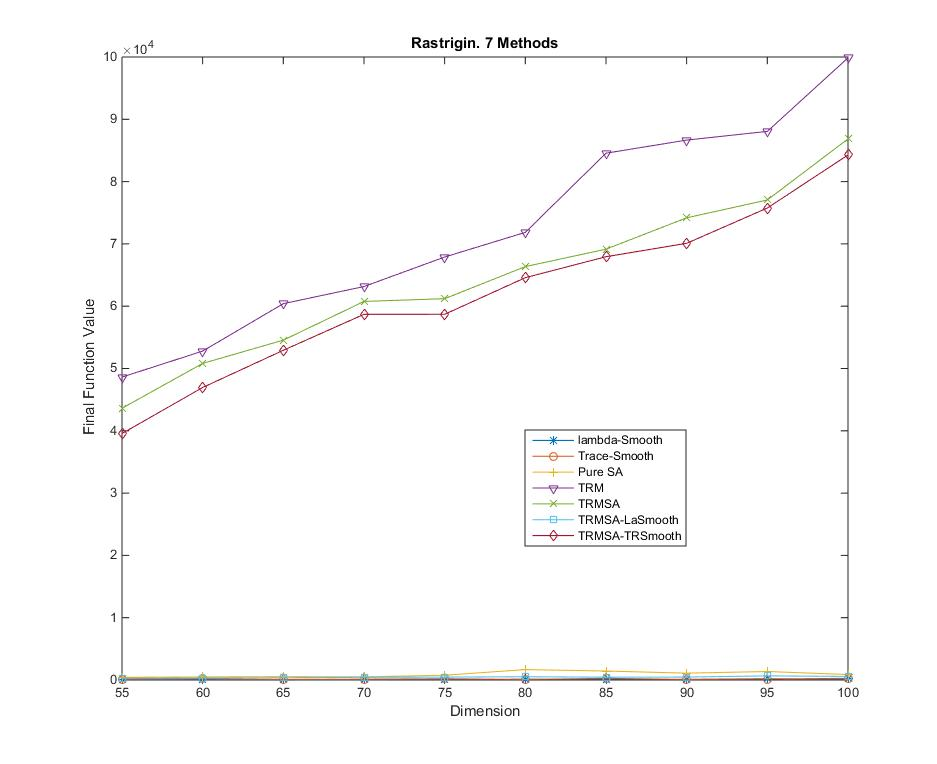
\includegraphics[scale=0.5]{rast7methods.jpg}
\caption{Rastrigin example. 7 Methods. $n=55$ to $100$}
\end{figure}

As we can see, traditional TRM, TRMSA and TRMSA with $Trace-Smooth$ do not give us a satisfied results. Probably because Rastrigin has many local optima and it is very difficult for TRM to solve. Also, since we just use the original function $f(x)$'s gradient and Hessian matrix so the TRMSA with $Trace-Smooth$ does not do well either. 

Below we show the plot of four methods which did quite well for this problem (the ones of bottom lines): Pure SA, SA with $Trace-Smooth$, SA with $\lambda-Smooth$ and TRMSA with $\lambda-Smooth$.

\begin{figure}[H]
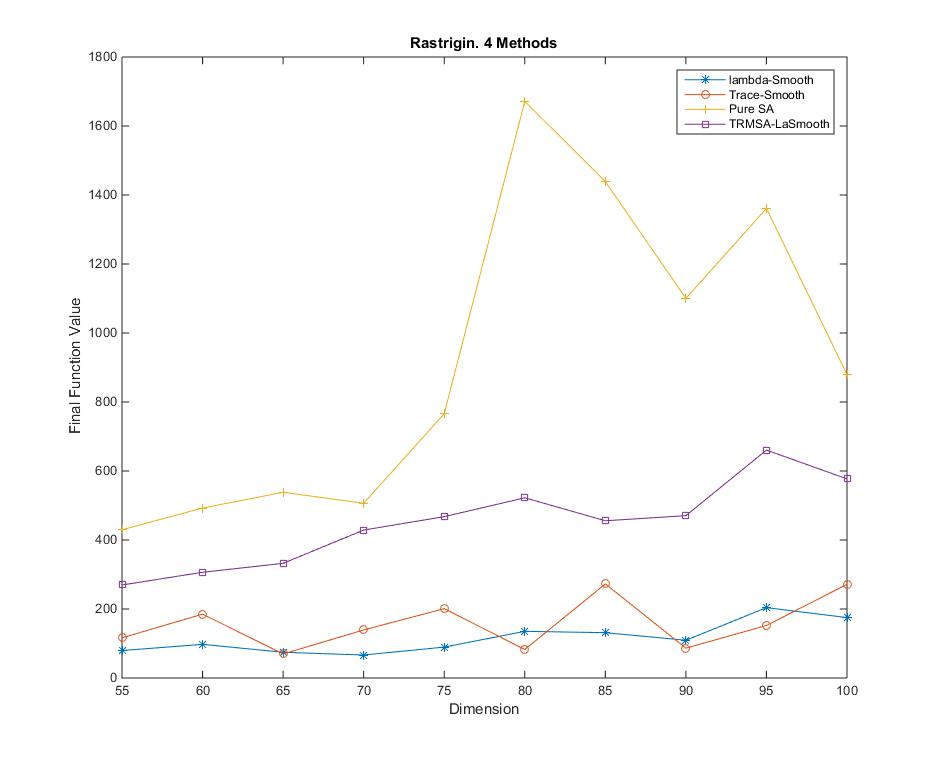
\includegraphics[scale=0.5]{rast4methods.jpg}
\caption{Rastrigin example. 4 Methods. $n=55$ to $100$}
\end{figure}

Now we can give a conclusion which is: for those problems that have many local optima, TRM, TRMSA and TRMSA with $Trace-Smooth$ probably can not do well. For the rest 4 methods that can do quite well in those problems, Pure SA may be the worst, and SA with $Trace-Smooth$ and SA with $\lambda-Smooth$ can do best. TRMSA with $\lambda-Smooth$ is between them.

Now we show the results of solving the optimization problem for Griewank and modified Griewank function. In this case, the problem is not so difficult to solve, so the difference between our 7 methods is not so big but we can see the conclusions we drew before still hold.

\begin{figure}[H]
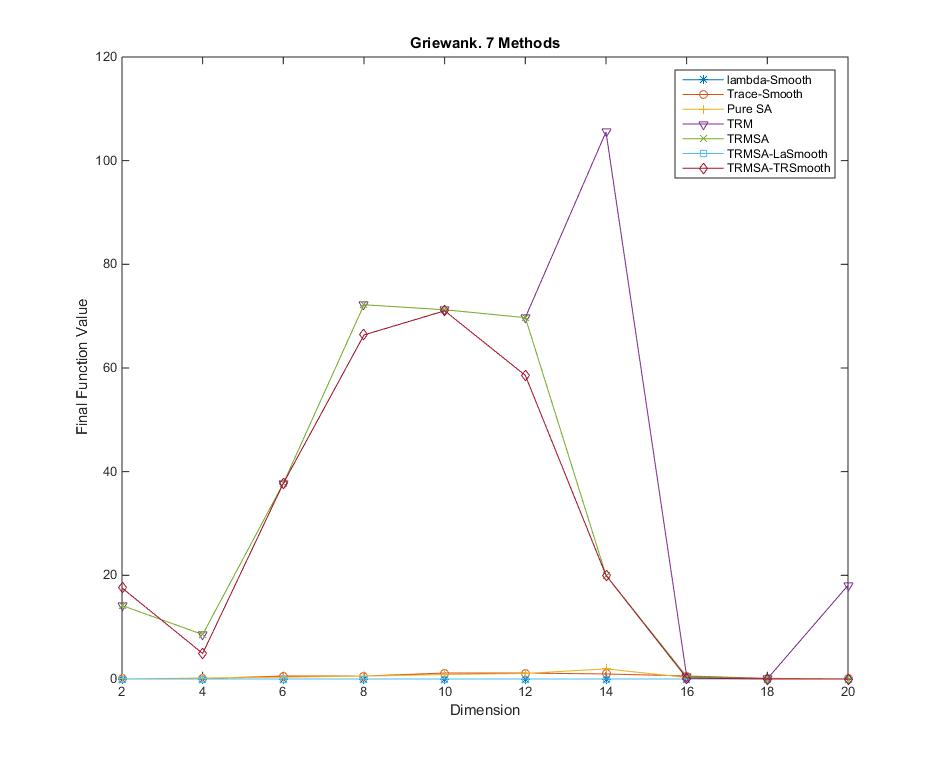
\includegraphics[scale=0.5]{griewank7methods.jpg}
\caption{Griewank example. 7 Methods. $n=2$ to $20$}
\end{figure}

\begin{figure}[H]
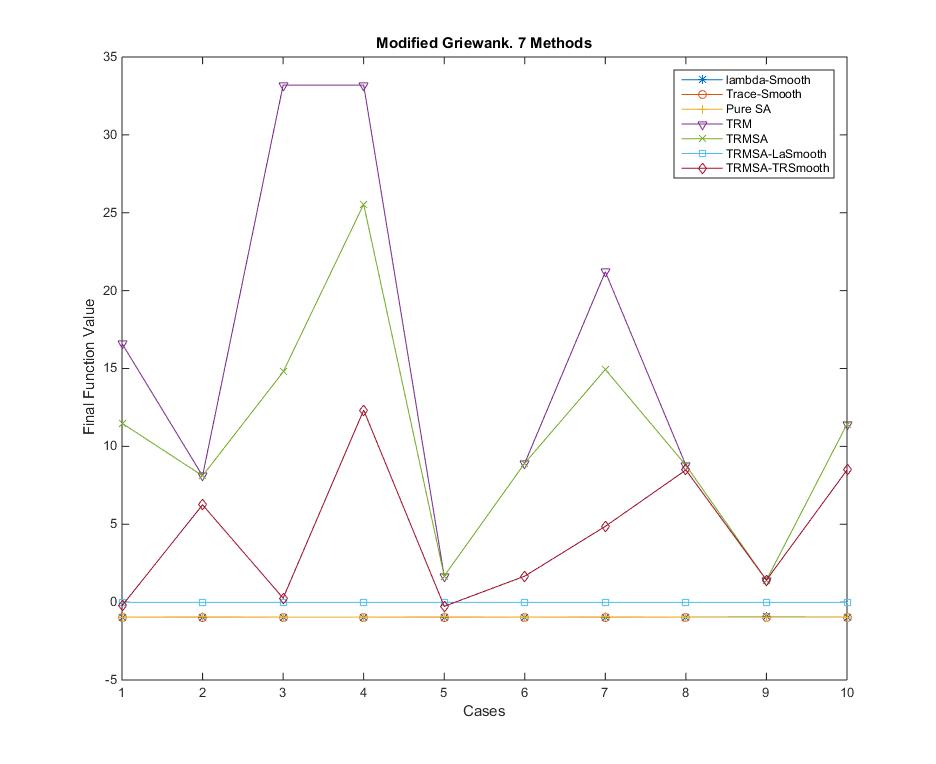
\includegraphics[scale=0.5]{griewank27methods.jpg}
\caption{Modified Griewank example. 7 Methods. $n=2$. 10 Cases}
\end{figure}
After doing these experiments, we move forward to focus on 4 methods: 

\begin{itemize}

\item SA with $Trace-Smooth$

\item SA with $\lambda-Smooth$

\item TRMSA with $\lambda-Smooth$

\item TRM with $\lambda-Smooth$

\end{itemize} 

The last one is a new method cause we find it takes much fewer evaluations of $f(x)$ and Hessian matrix but can still get a good result. And the algorithm is :

\begin{algorithm} [H]
\caption{Trust-Region Method with $\lambda-Smooth$}
\begin{algorithmic} 
\STATE Given $x_0$, $m=0$, $x_*$, $\lambda$ sequence:$Ls$.
\STATE \emph{Phase 1:}
\FOR {$ l =1,...,length(Ls)$}
\STATE Given $\tau_1, \tau_2, \gamma1, \gamma2$, $\lambda=Ls(l)$
\WHILE {$norm(g)>tol$ and number of iterations$<itbnd$}
\STATE  Solve TRS for $s_k$ with $\bar{g}=g+2\lambda(x-x_*)$ and $\bar{H}=H+2\lambda I$, assign $qpval_k \leftarrow \triangledown  f^T_ks_k+\frac{1}{2}s^T_k \triangledown^2f_ks_k$
\STATE  $newval_k\leftarrow f(x_k+s_k)+\lambda||x_k+s_k-x_*||_2^2$
\STATE  $ratio_k\leftarrow \frac{newval_k-(f_k+\lambda||x_k-x_*||_2^2)}{qpval_k}$
\STATE  Adjust $\Delta_k$
\IF{ $ratio_k< \tau_1$} 
\STATE $\Delta_{k+1}\leftarrow \frac{||s_k||}{\gamma_1}$
\ELSE 
\IF{$ratio_k>\tau_2$,and $||s_k||=\Delta_k$}
\STATE $\Delta_{k+1}\leftarrow \gamma_2 \Delta_k$
\ELSE 
\STATE $\Delta_{k+1}\leftarrow \Delta_k$
\ENDIF
\ENDIF
\STATE Update $x$:
\IF {$ratio_k\geq 0$}
\STATE $x_{k+1}\leftarrow x_k+s_k$
\ELSE 
\STATE $x_{k+1}\leftarrow x_k$
\ENDIF
\ENDWHILE
\STATE $f_n=f(x_k)$
\IF{ $f_n$ is different from any $f_1$ to $f_{n-1}$} 
\STATE $m=m+1$, $\overline{x_m}=x_k$, ;
\ENDIF
\ENDFOR
\STATE  
\STATE \emph{Phase 2:}
\FOR {$k=1,...,m$}
\STATE Algorithm 4 with initial point $\overline{x_k}$
\ENDFOR
\STATE Output the smallest $f$ in phase 2 and its point.
\end{algorithmic}
\end{algorithm}

Now we give some results about these 4 methods.

\begin{figure}[H]
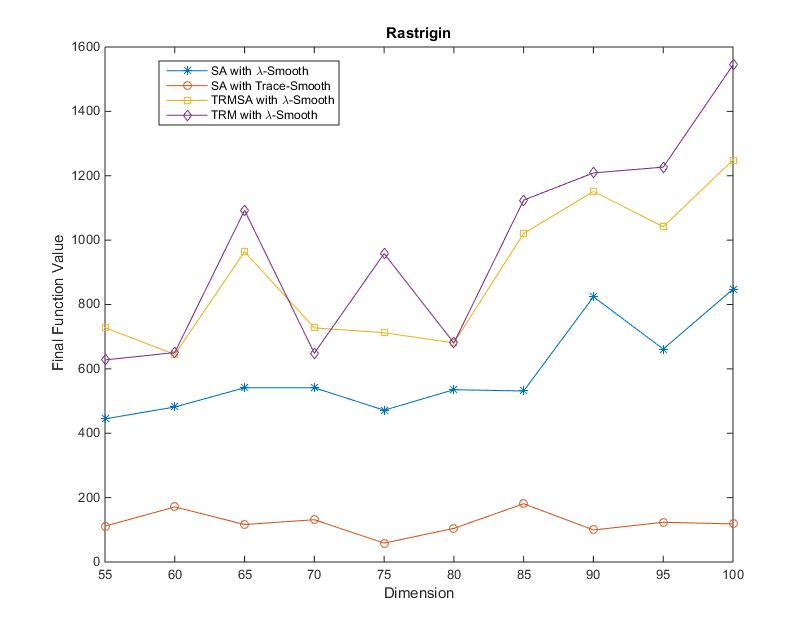
\includegraphics[scale=0.6]{rast4methods2.jpg}
\caption{Rastrigin. 4 Methods. $n=55$ to $100$}
\end{figure}

Below we show the number of evaluation of function value and Hessian matrix. For each method, the left number shows the number of evaluation of function value and the right one is for Hessian matrix. Notice that Tr means $Trace-Smooth$ and La means $\lambda-Smooth$. We randomly generated $x_*$ from $[-5,5]^n$ for all $\lambda-Smooth$ method and we know the global optimum is $[0,0,...,0]$.

\begin{lstlisting}

 Dim     SAwithLa        SAwithTr      TRMSAwithLa     TRMwithLa  
 ___    __________    _____________    ___________    ___________

  55    80412    0    80414   80412    3576   3575     627    626
  60    80415    0    80412   80410    3152   3151    1116   1115
  65    80412    0    80413   80411    3149   3148    1597   1596
  70    80414    0    80418   80416    3528   3527     647    646
  75    80416    0    80415   80413    3079   3078    1110   1109
  80    80415    0    80416   80414    4533   4532     610    609
  85    80413    0    80413   80411    3189   3188     679    678
  90    80416    0    80415   80413    3522   3521     664    663
  95    80418    0    80415   80413    3565   3564     671    670
 100    80418    0    80417   80415    3287   3286    1605   1604
 
\end{lstlisting}

From the table we can see that the more information (function values and Hessian matrix) we use, the better answer we will get, which is reasonable.

\chapter{Summary}

\section{Advantage of SA+Smoothing}

\begin{itemize}

\item Doing better than $fmincon$(Trust-Region) method.

\item Take much less time and doing better than $simulannealbnd$(MATLAB build-in SA function).

\item Take a reasonable time to get final results (With user-supply Hessian Matrix).

\item The smoothing part really works.

\item $\lambda-Smooth$ can work well if we know the rough region of where global optimum locates.

\end{itemize}

\section{TRM with SA and Smoothing}

\begin{itemize}

\item TRM with SA and Smoothing is doing better than TRM with SA and traditional TRM.

\item TRM with SA and $Trace-Smooth$ does not so good as we expected since we cannot get the third and forth derivation information.

\item TRM with $\lambda-Smooth$ does almost the same as TRM with SA and $\lambda-Smooth$ but needs fewer evaluations of function values and Hessian matrix.

\item We can input several different $x_*$ if we want.

\item All parameters may infect the results, we should define them properly.

\item For TRM with SA and Smoothing, the temperature sequence can be much shorter than SA with smoothing. For SA, usually we use $Ts=T_0*0.9^{(0:199)}$. For TRM with SA and Smoothing, usually we use $Ts=10*0.3^{(0:4)}$

\item Need some more examples and test problems. For now we use Rastrigin for most cases because for the rest of test problems we have, the results of these methods probably show no difference. 

\end{itemize}

\section{Challenges}

\begin{itemize}

\item $\Delta$-sequence for $Trace-Smooth$ is really important for the method, but it's a little difficult to find it perfect cause it depends on the problem. However, we have a certain way to compute it but it needs more test and proof. 

\item Including all challenges in simulated annealing, which means the parameter settings and so on.

\item The $\lambda-Smooth$ technique can work well in the condition that we know where the global optimum locates.

\item If we use $ADMAT$ to compute $H$, it will take a much longer time.

\item SA with $Trace-Smooth$ is sensitive to the parameters.

\end{itemize}

\section{Further Work}

\begin{itemize}

\item Need more examples and test problems.

\item How to decide the $\Delta$ or $\lambda$ sequence precisely.

\item For SA with $Trace-Smooth$ we may think another way to compute part of $H$ cause we only need the trace of $H$.

\end{itemize}

\section{Existing Codes}

The algorithm codes for our experiments includes:

\begin{itemize}

\item PureSA - Pure simulated annealing algorithm.

\item SmoothSA - Simulated annealing with $\lambda-Smooth$ algorithm.

\item SmoothTraceSA - Simulated annealing with $Trace-Smooth$ algorithm.

\item TRM - Traditional trust-region method.

\item TRMSA - Trust-region method with simulated annealing.

\item TRMSALaSmooth - Trust-region method with simulated annealing and $\lambda-Smooth$.

\item TRMSATrSmooth - Trust-region method with simulated annealing and $Trace-Smooth$.

\item TRMLaSmooth - Trust-region method with $\lambda-Smooth$.

\item Trust, trust3 - Solve trust-region sub-problem, these 2 codes are from mathwork.

\item neighbor - Compute neighborhood. It is from CGO package.

\end{itemize}

\section{Test Problems and Contact Information}

There are several test problems in the package, most of them come from the website:
\url{http://www.sfu.ca/~ssurjano/optimization.html} and CGO package.

If you have any questions or concerns about this report, please contact Yichen ZHANG through \href{mailto:yichen.zhang@uwaterloo.ca}{yichen.zhang@uwaterloo.ca}

\end{document} 